\chapter{Optimizaciones software para acelerar el muestreo de distribuciones} \label{ch:optimizaciones}

A continuación se presentan 2 propuestas de aceleración software con distribuciones Bernoulli y Uniformes como candidatas a sustituir a distribuciones Gaussianas, ya que muestrear estas últimas es más costoso.

\section{Distribuciones Bernoulli}

Awano \emph{et al.} propusieron muestrear distribuciones Bernoulli en vez de distribuciones Gaussianas para aumentar la eficiencia del algoritmo en un acelerador para inferencia \cite{bnn_clt_approx}. Los parámetros de estas nuevas distribuciones se obtienen mediante una transformación de los parámetros de las distribuciones originales. En este trabajo se ha implementado esta optimización mediante software y se ha analizado su impacto en la precisión, métricas de incertidumbre y rendimiento. A continuación se explican los fundamentos teóricos de la optimización.

El TCL expone que en condiciones generales la distribución de una suma de variables aleatorias tiende a ser una distribución gaussiana. Las operaciones MAC son una suma de variables aleatorias por lo que según el TCL el resultado seguirá una distribución gaussiana. Una distribución gaussiana se define con 2 parámetros, la media y la desviación típica. Asumiendo que el tipo de distribución resultante es independiente del tipo de distribuciones de los sumandos, solamente se tiene que preservar la esperanza y la varianza de la operación MAC para no alterar los resultados de la BNN. Las Ecuaciones \ref{eq:neuron_expected}  y \ref{eq:neuron_variance} muestran la esperanza y la varianza de una operación MAC.
\begin{equation} \label{eq:neuron_expected}
E\left[ b + \sum_{i=0}^N w_i x_i \right]  = b + \sum_{i=0}^N ( E[w_i] E[x_i] )
\end{equation}
\begin{equation} \label{eq:neuron_variance}
V\left[ b + \sum_{i=0}^N w_i x_i \right] = \sum_{i=0}^N ( V[w_i]V[x_i] + V[w_i]E[x_i]^2 + V[x_i]E[w_i]^2 )
\end{equation}

La optimización consiste en utilizar un nuevo peso $w'$ que cumpla $E[w'] = E[w]$ y $V[w'] = V[w]$, de forma que no altere los resultados de la BNN. Se define $w' = qb$, siendo $b$ una muestra de una distribución Bernoulli $\mathcal{B}(p)$, esta distribución toma el valor 1 con probabilidad $p$ y el valor 0 con probabilidad $1-p$. Las constantes $p$ y $q$ se calculan a partir de la media $\mu$ y desviación típica $\sigma$ de las distribuciones originales mediante el sistema de ecuaciones mostrado en la Ecuación \ref{eq:bernoulli_opt}.
\begin{equation}\label{eq:bernoulli_opt}
\begin{cases}
\mu = pq\\ \\
\sigma^2 = p(1-p)q^2
\end{cases}
\rightarrow\ 
\begin{cases}
p = \dfrac{\mu^2}{\mu^2 + \sigma^2}\\ \\
q = \dfrac{\mu^2 + \sigma^2}{\mu}
\end{cases}
\end{equation}

Esta optimización no aumenta el tamaño de los modelos y no necesita muestrear distribuciones gaussianas sino Bernoulli, cuyo algoritmo de muestreo es mucho más sencillo. Dicho algoritmo de muestreo incluye una instrucción de salto, este tipo de instrucciones puede tener un coste muy elevado en algunas arquitecturas hardware. Por lo que este trabajo ha desarrollado otra optimización que utiliza una distribución que no requiere este tipo de instrucciones, explicada a continuación.

\section{Distribuciones Uniformes}

Partiendo de Awano \emph{et al.} este trabajo propone un nuevo método que utiliza distribuciones Uniformes en vez de distribuciones Bernoulli. En este caso el nuevo peso se define como $w' = bu + a$, siendo $u$ una muestra de una distribución Uniforme $\mathcal{U}(0,1)$. $a$ y $b$ siendo constantes que se pueden calcular a partir de la media $\mu$ y desviación típica $\sigma$ de los pesos originales utilizando el sistema de ecuaciones mostrado en la Ecuación \ref{eq:uniform_opt}.
\begin{equation}\label{eq:uniform_opt}
\begin{cases}
\mu = \dfrac{b}{2} + a\\ \\
\sigma^2 = \dfrac{b^2}{12}
\end{cases}
\rightarrow\ 
\begin{cases}
a = \mu - \dfrac{b}{2}\\ \\
b = \sigma \sqrt{12}
\end{cases}
\end{equation}

Esta optimización tampoco aumenta el tamaño de los modelos, muestrea distribuciones Uniformes cuyo algoritmo de muestreo es muy sencillo y además no requiere instrucciones de salto.

\section{Análisis de resultados}

La Tabla \ref{tab:uniform_opt} muestra los resultados de precisión y aceleración (\textit{speedup}) obtenidos con las optimizaciones Bernoulli y Uniforme para todas las arquitecturas de modelos y conjuntos de datos.

\begin{table}[h]
    \centering
    \caption{Resultados de precisión y \textit{speedup} obtenidos con las optimizaciones Bernoulli y Uniforme para todas las arquitecturas de modelos y conjuntos de datos.}
    \label{tab:uniform_opt}
    \begin{tabular}{llrrrrr}
    \hline
     \multirow{2}{*}{\textbf{Modelo}} & \textbf{Conjunto} & \multicolumn{3}{c}{\textbf{Precisión}} & \multicolumn{2}{c}{\textbf{Speedup}} \\
     
     & \multicolumn{1}{c}{\textbf{de datos}} & \multicolumn{1}{l}{\textit{TensorFlow}} & \multicolumn{1}{l}{\textit{Bernoulli}} & \multicolumn{1}{l}{\textit{Uniforme}} & \multicolumn{1}{l}{\textit{Bernoulli}} & \multicolumn{1}{l}{\textit{Uniforme}} \\ \hline
    \multirow{5}{*}{HYPER} 
        & BO & 0.9039 & 0.9039 & 0.9082 & \multirow{5}{*}{5.18} & \multirow{5}{*}{4.95} \\
        & IP & 0.8139 & 0.8154 & 0.8130 \\
        & KSC & 0.9256 & 0.9274 & 0.9217 \\
        & PU & 0.9017 & 0.9004 & 0.9016 \\
        & SV & 0.9257 & 0.9238 & 0.9279 \\ \hline
    \multirow{2}{*}{LENET-5} 
        & MNIST & 0.9836 & 0.9883 & 0.9885 & \multirow{2}{*}{4.28} & \multirow{2}{*}{3.87} \\
        & CIFAR-10 & 0.6351 & 0.6336 & 0.6220 & \\ \hline
    \multirow{2}{*}{B2N2} 
        & MNIST & 0.9872 & 0.9917 & 0.9910 & \multirow{2}{*}{5.67} & \multirow{2}{*}{5.64} \\
        & CIFAR-10 & 0.7295 & 0.7273 & 0.7197 & \\ \hline                  
    \end{tabular}
\end{table}

Ninguna de las optimizaciones tiene un efecto negativo en la precisión de los modelos utilizados para verificación. Si el muestreo de la distribución Bernoulli devuelve 0 se pueden ignorar el resto de instrucciones de la operación MAC de dicho operando, ya que acumularía 0. Esto lo hace el compilador de forma automática en la fase de optimización de eliminación de código muerto. En el caso del procesador RISC-V utilizado la penalización de las instrucciones de salto es solamente de 2 ciclos, por lo que debido a esto junto con la eliminación de código la optimización Bernoulli obtiene un \textit{speedup} mayor que la Uniforme.

Con respecto a la preservación de las métricas de incertidumbre, ambas optimizaciones producen pequeñas alteraciones. La magnitud de estas alteraciones es dependiente de la optimización y del modelo, en algunos casos la optimización Bernoulli produce alteraciones menores y en otros la Uniforme. La Figura \ref{fig:comp_lenet_cifar} muestra un caso en el que la optimización Bernoulli produce menos alteraciones que la Uniforme y la Figura \ref{fig:comp_bo} un caso en el que ocurre lo contrario. Se ha considerado que estas variaciones son pequeñas y no llegan a tener un efecto negativo en la utilidad de las métricas.

En el Anexo \ref{anx:bernoulli} se pueden encontrar los resultados obtenidos con todos los modelos y conjuntos de datos utilizando la optimización Bernoulli y en el Anexo \ref{anx:uniforme} utilizando la optimización Uniforme.


\begin{figure}[h]
    \begin{subfigure}[b]{0.49\textwidth}
         \centering
         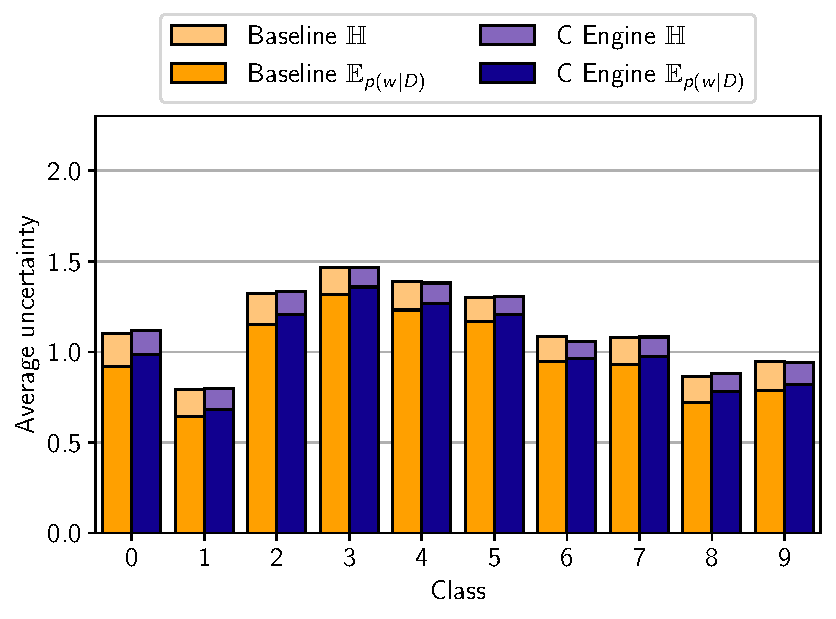
\includegraphics[width=\textwidth]{root/Imagenes/opt_software/Bernoulli/LENET_CIFAR/class_uncertainty.pdf}
         \caption{Optimización Bernoulli}
    \end{subfigure}
    \hfill
    \begin{subfigure}[b]{0.49\textwidth}
         \centering
         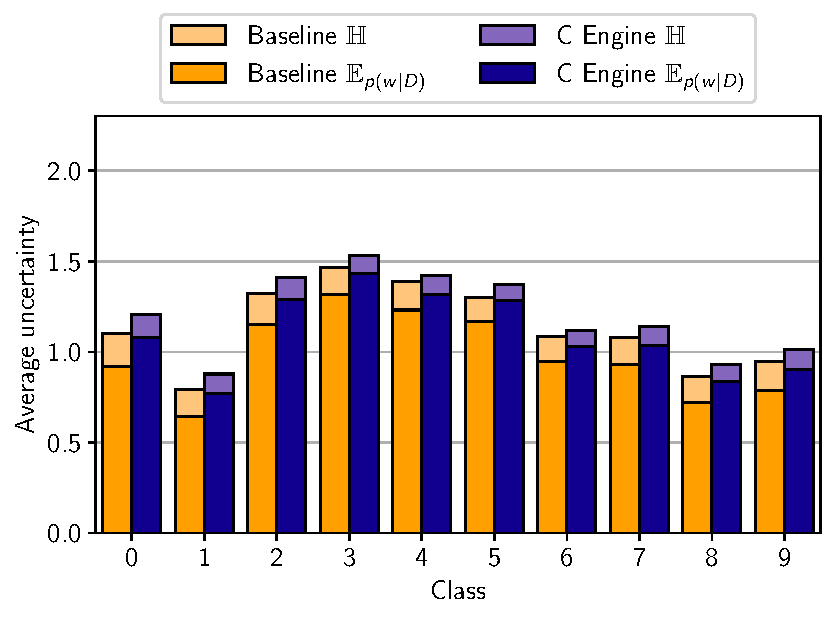
\includegraphics[width=\textwidth]{root/Imagenes/opt_software/Uniform/LENET_CIFAR/class_uncertainty.pdf}
         \caption{Optimización Uniforme}
    \end{subfigure}
    \caption{Incertidumbre predictiva ($\mathbb{H}$) y aleatoria ($\mathbb{E}p$) agrupada por clases de las predicciones obtenidas con \textit{TensorFlow} (amarillo) y el motor de inferencia optimizado (azul) del modelo LeNet-5 y el conjunto de datos CIFAR-10.}
    \label{fig:comp_lenet_cifar}
\end{figure}

\begin{figure}[h]
     \centering
     \begin{subfigure}[b]{0.49\textwidth}
         \centering
         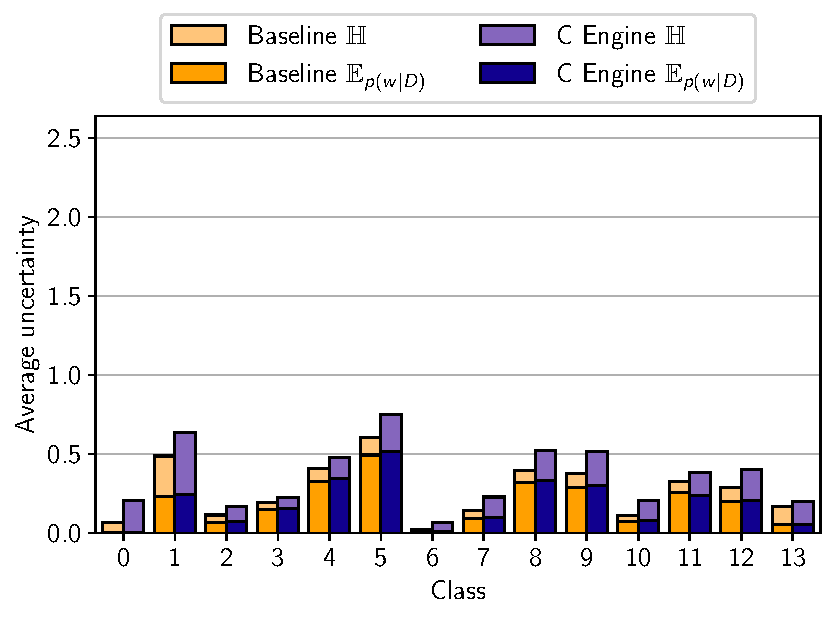
\includegraphics[width=\textwidth]{root/Imagenes/opt_software/Bernoulli/HYPER_BO/class_uncertainty.pdf}
         \caption{Optimización Bernoulli}
     \end{subfigure}
     \begin{subfigure}[b]{0.49\textwidth}
         \centering
         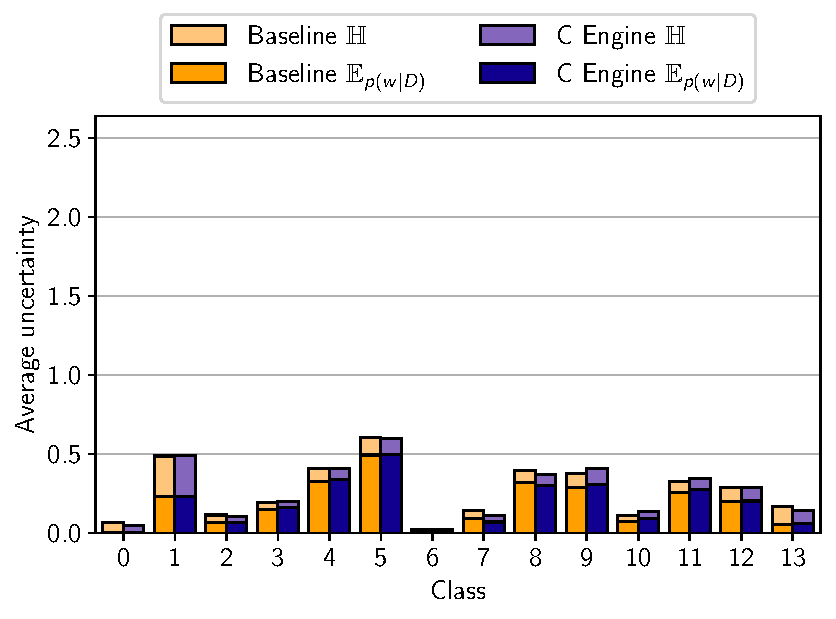
\includegraphics[width=\textwidth]{root/Imagenes/opt_software/Uniform/HYPER_BO/class_uncertainty.pdf}
         \caption{Optimización Uniforme}
     \end{subfigure}
    \caption{Incertidumbre predictiva ($\mathbb{H}$) y aleatoria ($\mathbb{E}p$) agrupada por clases de las predicciones obtenidas con \textit{TensorFlow} (amarillo) y el motor de inferencia optimizado (azul) del conjunto de datos de píxeles hiperespectrales BO.}
    \label{fig:comp_bo}
\end{figure}

